\documentclass{beamer}
\usepackage[T1]{fontenc}

\usepackage{polski}
\usepackage[utf8]{inputenc}
\usepackage[polish]{babel}
%
% Choose how your presentation looks.
%
% For more themes, color themes and font themes, see:
% http://deic.uab.es/~iblanes/beamer_gallery/index_by_theme.html
%
\mode<presentation>
{
	\usetheme{Warsaw}      % or try Darmstadt, Madrid, Warsaw, ...
	\usecolortheme{crane} % or try albatross, beaver, crane, ...
	\usefonttheme{default}  % or try serif, structurebold, ...
	\setbeamertemplate{headline}{}
	\setbeamertemplate{caption}[numbered]
} 

\title[Praca magisterska]{Rekomendacje artykułów opisujących produkty w serwisach e-commerce}
\author{Łukasz Dragan}
\institute{Informatyka spec. Metody sztucznej inteligencji, MiNI PW}
\date{31.10.2017}

\begin{document}
	
	\begin{frame}
		\titlepage
	\end{frame}
	
	\begin{frame}{Plan prezentacji}
	  \tableofcontents
	\end{frame}
	
	\section{Cel pracy}
		\begin{frame}{Cel pracy}
			Czy metody semantycznej analizy tekstu mogą być alternatywą dla~dotychczas uzywanej przez~\emph{Allegro} metody generowania rekomendacji artykułów tekstowych?
		\end{frame}
	\section{Opis problemu}
	
	\begin{frame}{pracuj.pl}
		\begin{figure}
			\centering
			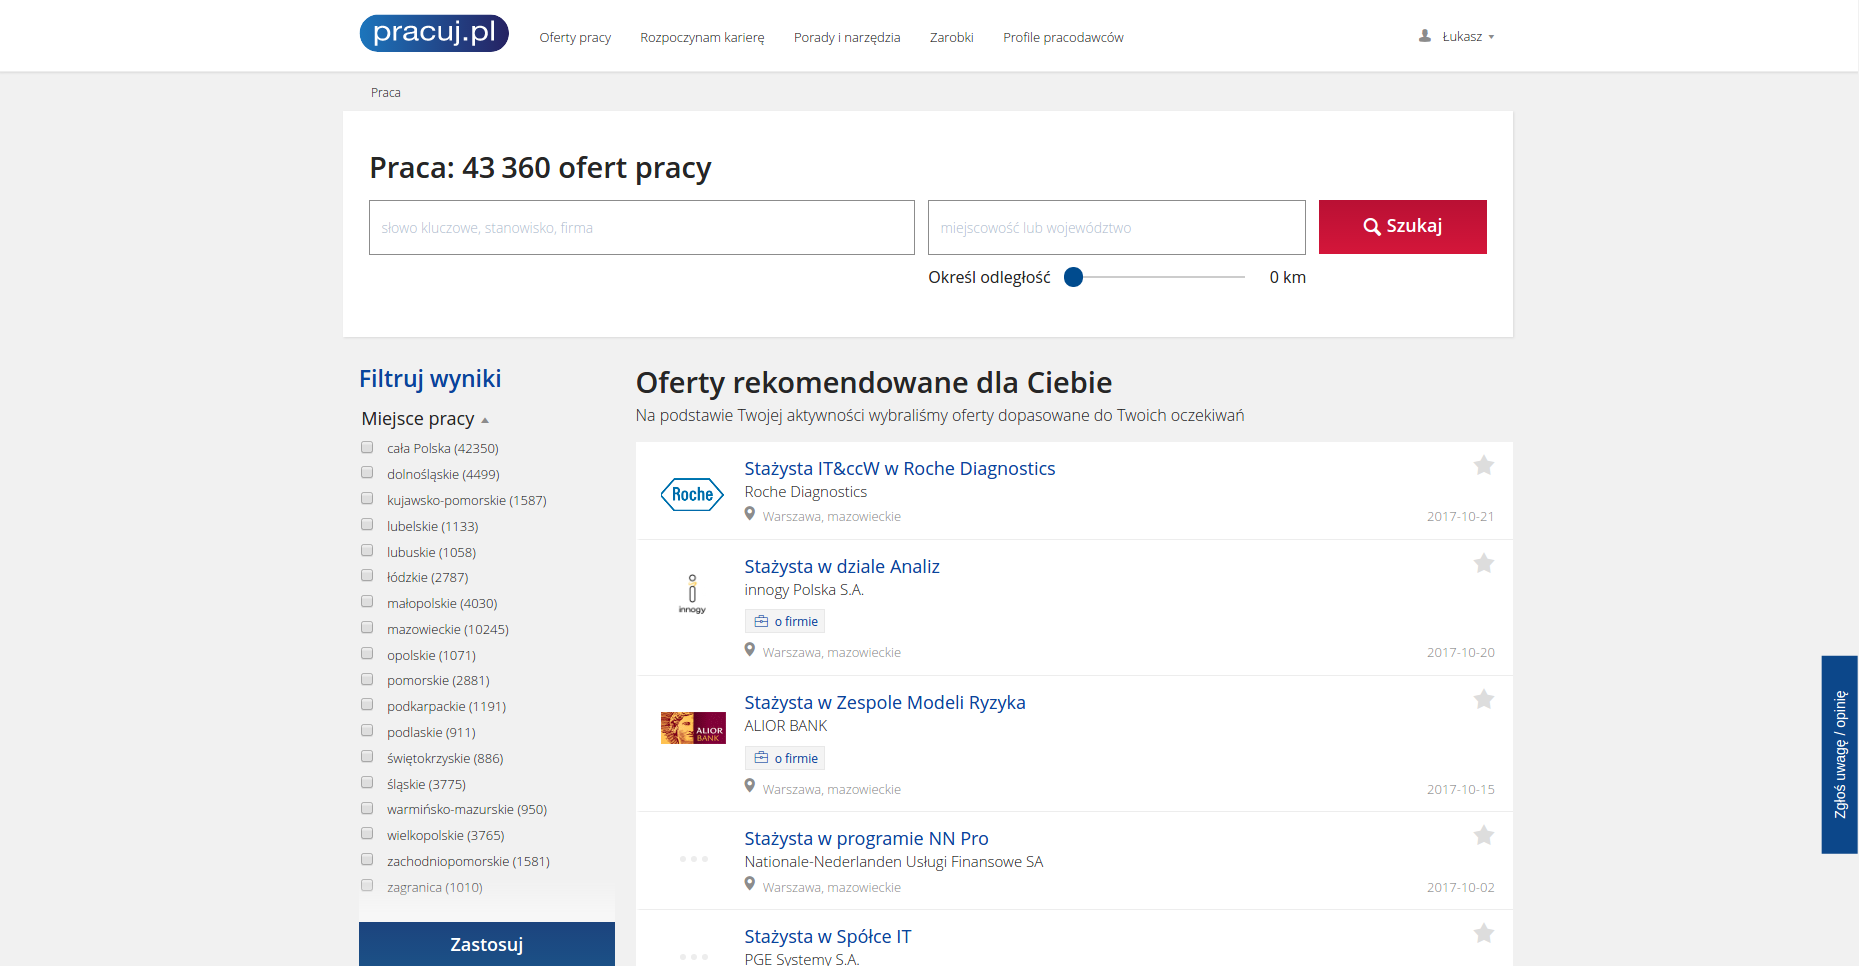
\includegraphics[width=1\textwidth]{img/pracuj.png}
		\end{figure}
	\end{frame}
	
	\begin{frame}{filmweb.pl}
		\begin{figure}
			\centering
			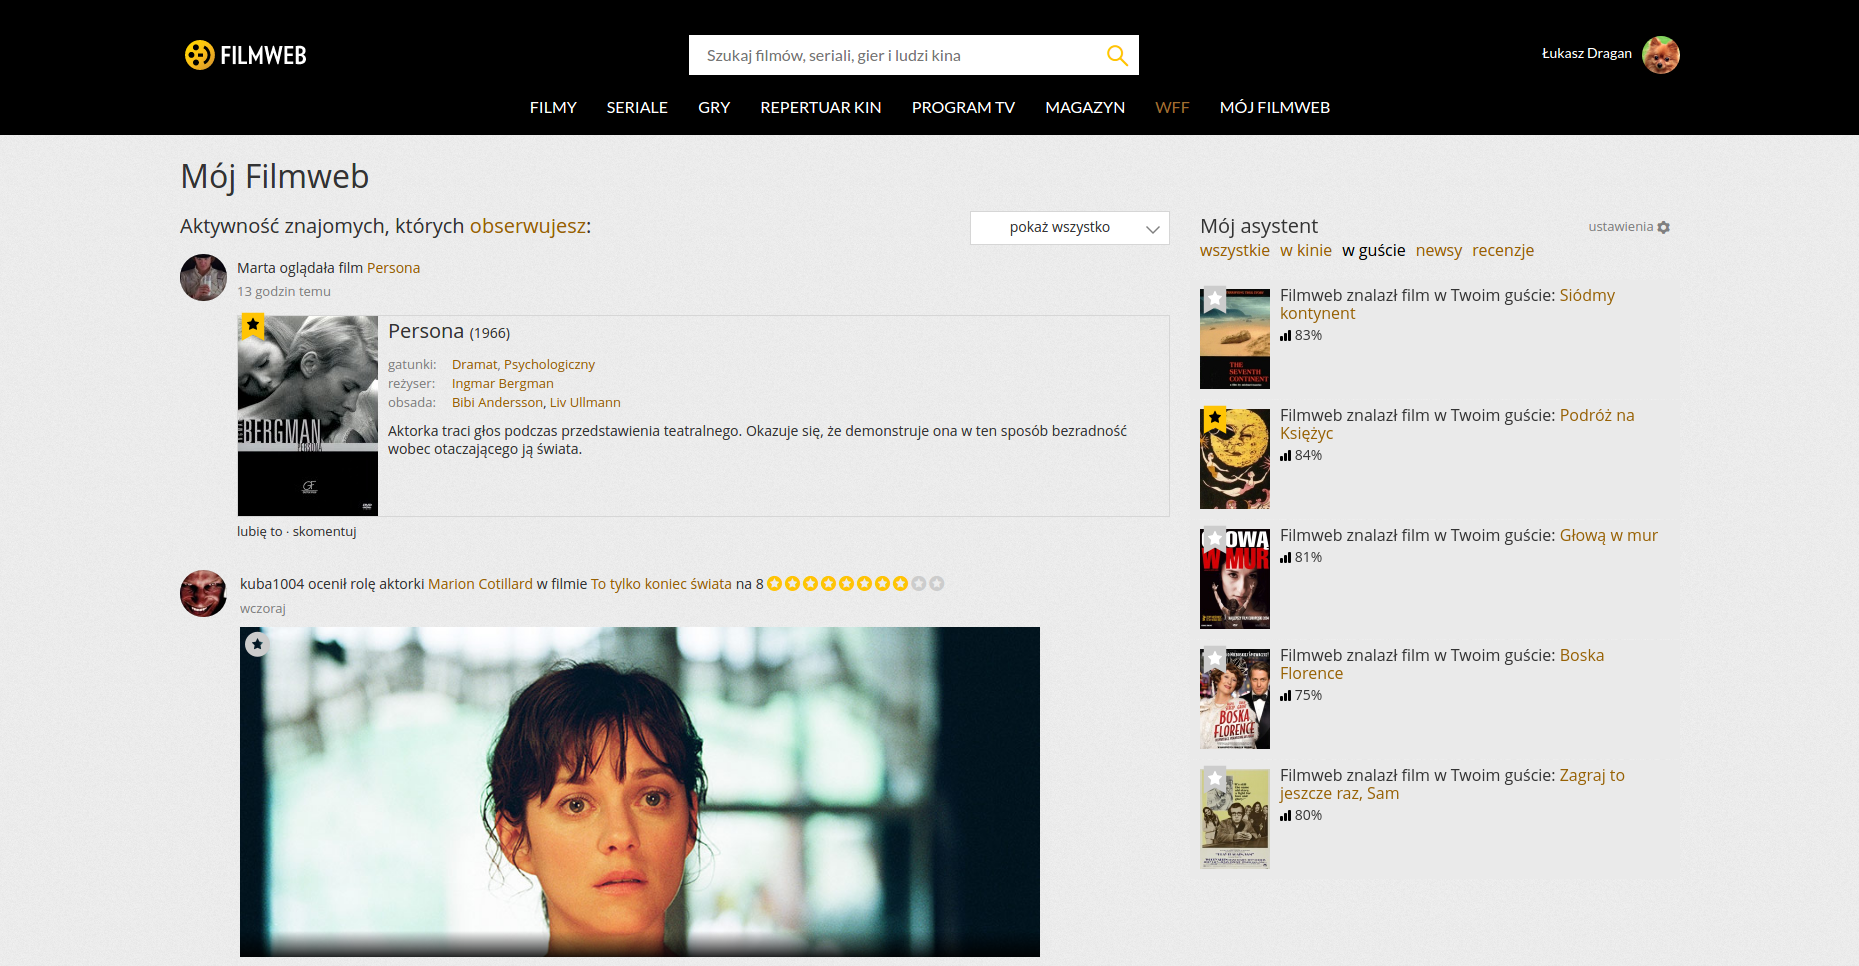
\includegraphics[width=1\textwidth]{img/filmweb.png}
		\end{figure}
	\end{frame}
	
	\begin{frame}{allegro.pl}
		\begin{figure}
			\centering
			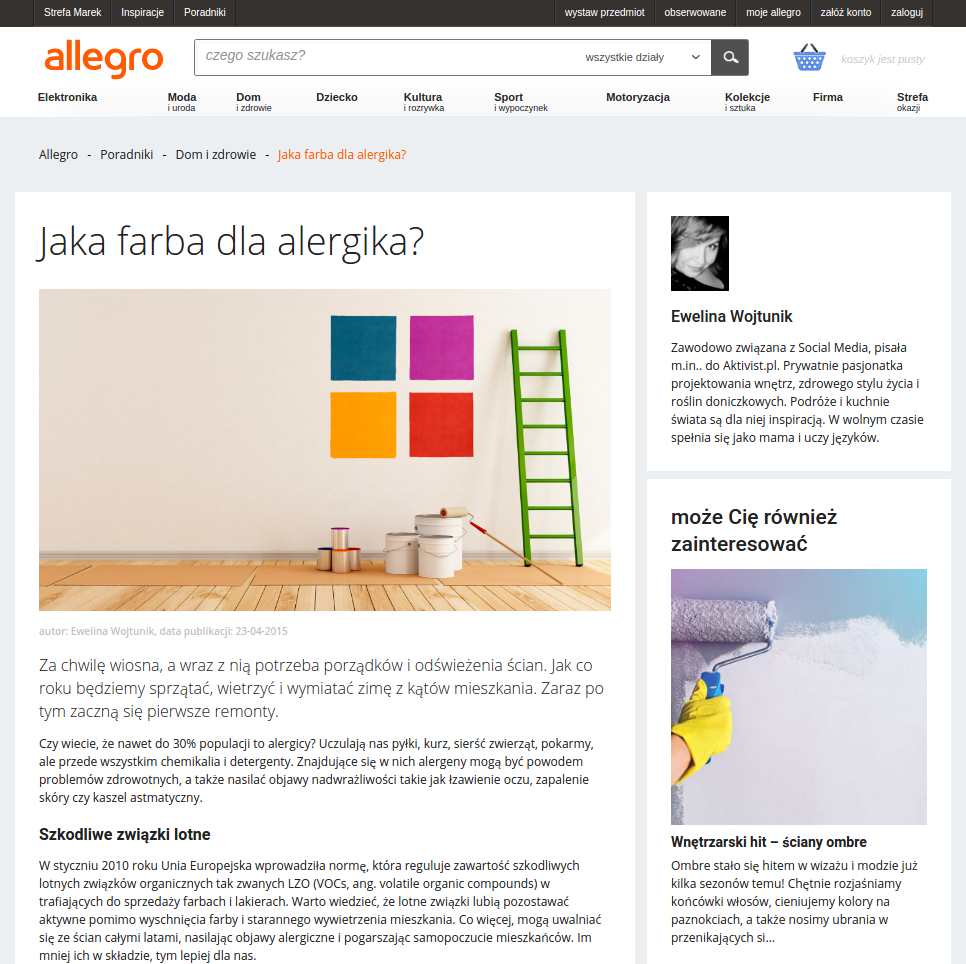
\includegraphics[width=1\textwidth]{img/screen_allegro.png}
		\end{figure}
	\end{frame}
	
	\begin{frame}{allegro.pl cd}
		\begin{figure}
			\centering
			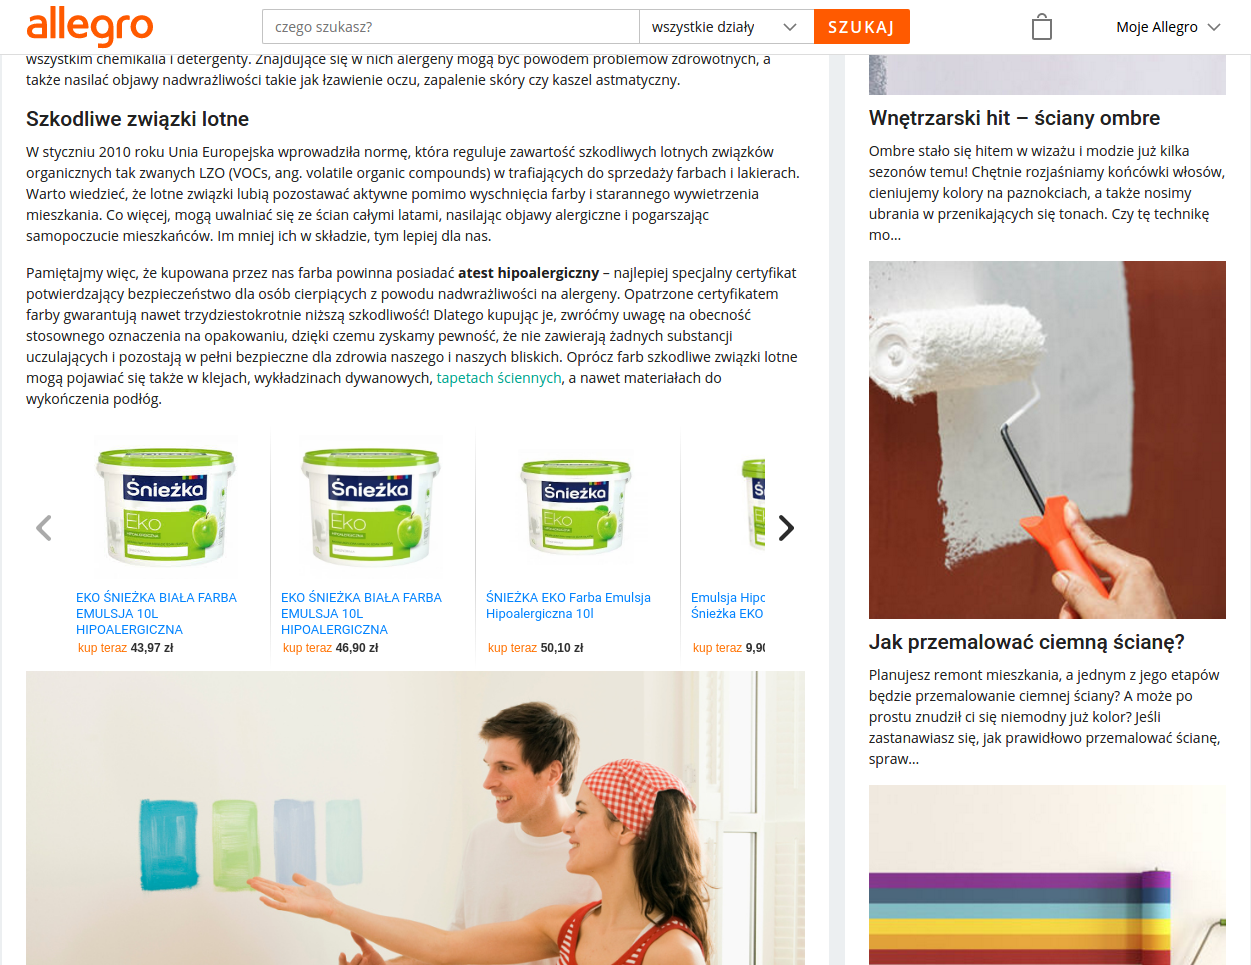
\includegraphics[width=1\textwidth]{img/screen_allegro_2.png}
		\end{figure}
	\end{frame}
	
	\section{Systemy rekomendacji}
	\begin{frame}{Elasticsearch}
		\begin{figure}
			\centering
			
\includegraphics[width=0.5\textwidth]{img/elastic-logo.png}
		\end{figure}
		,,Elasticsearch is a distributed, JSON-based search and analytics engine designed for horizontal scalability, maximum reliability, and easy management.''
	\end{frame}

	\begin{frame}{Systemy rekomenadacji}
		%TODO
		W ujęciu ogólnym systemy wyszukiwania mają na~celu sugerowanie tego, co użytkownik chciałby otrzymać. Natomiast systemy rekomendacji mają sugerować przedmioty potrzebne użytkownikowi nawet, jeżeli potrzeby te nie~zostały bezpośrednio wyrażone.
	\end{frame}
	
	\begin{frame}{Systemy rekomenadacji}
		\begin{figure}
			\centering
			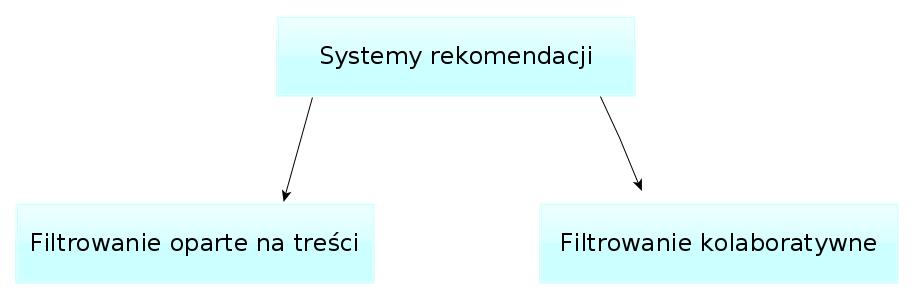
\includegraphics[width=1\textwidth]{img/recommender.png}
		\end{figure}
	\end{frame}
	\section{Techniki przetwarzania języka naturalnego}
	\begin{frame}{Zarys podejścia}
		\begin{figure}
			\centering
			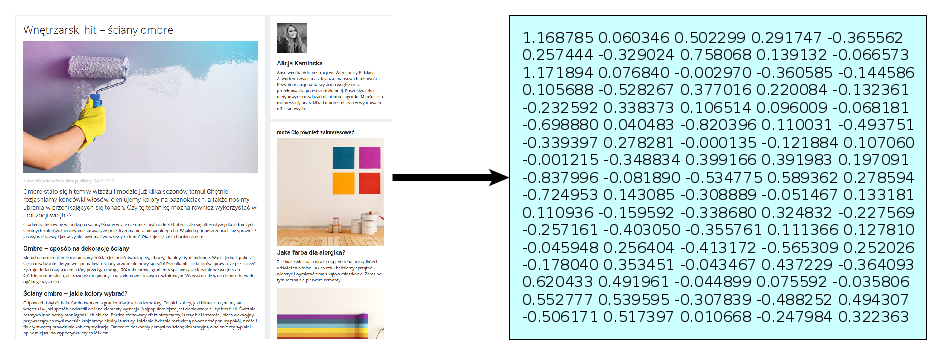
\includegraphics[width=0.85\textwidth]{img/approach_outline.png}
		\end{figure}
		\pause
		\begin{figure}
			\centering
			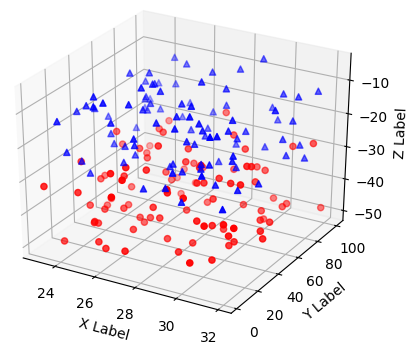
\includegraphics[width=0.45\textwidth]{img/scatter3d_demo.png}
		\end{figure}
	\end{frame}
	\subsection{Bag-of-words}
	\begin{frame}{Bag-of-words}
		\begin{figure}
			\centering
			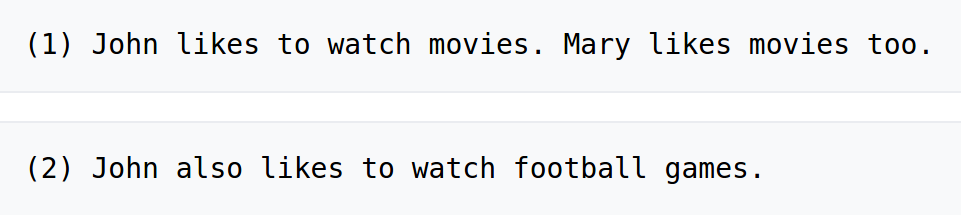
\includegraphics[width=0.75\textwidth]{img/bow_sents.png}
		\end{figure}
		\pause
		\begin{figure}
			\centering
			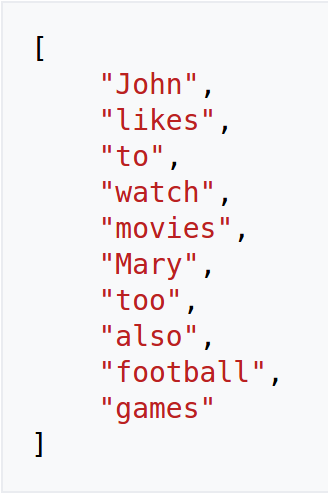
\includegraphics[width=0.25\textwidth]{img/bow_dict.png}
		\end{figure}
		\pause
		\begin{figure}
			\centering
			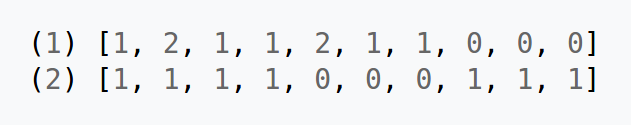
\includegraphics[width=0.5\textwidth]{img/bow_repr.png}
		\end{figure}
	\end{frame}
	\begin{frame}{Bag-of-words}
		Wady i zalety
	\end{frame}
	\subsection{TF-IDF}
	\begin{frame}{TF – term frequency, IDF – inverse document frequency}
		Wartość \textit{TF-IDF} słowa $w_i$ w dokumencie $d_j$:
		\begin{equation}
		\label{eq:tf-idf}
		tfidf_{ij} = tf_{ij} * idf_i,\ tf_{ij} = \frac{n_{ij}}{\sum\limits_{k}n_{kj}},\ idf_i = log\frac{|D|}{|{d:w_i \in d}|}
		\end{equation}
		\begin{itemize}
			\item $tf_{ij}$: liczba wystąpień słowa $w_i$ w~dokumencie $d_j$ podzielona przez~liczbę słów dokumentu $d_j$,
			\item $idf_i$: liczba dokumentów w~korpusie podzielona przez~liczbę dokumentów zawierających przynajmniej jedno wystąpienie słowa $w_i$.
		\end{itemize}
	\end{frame}
	\begin{frame}{TF-IDF}
		Przykład analogiczny do bow
	\end{frame}
	\begin{frame}{TF-IDF}
		Wady i zalety
	\end{frame}
	\subsection{Latent semantic analysis}
	\subsection{Latent Dirichlet allocation}
	\subsection{Word2vec}
	\begin{frame}
		rysunek z wektorami
	\end{frame}
	\subsection{FastText}
	\subsection{GloVe}
	
	
	\section{Opis danych}
	brak oryginalnych przykładów, bo podpisałem NDA
	\subsection{Zawartość artykułu}
	\begin{frame}
		jeszcze raz screen
	\end{frame}
	\subsection{Wstępne przetwarzanie danych}
	\begin{frame}
		\begin{enumerate}
			\item Oczyszczanie tekstu ze znaczników \pause
			\item Usunięcie słów stopu
		\end{enumerate}
	\end{frame}
	\begin{frame}{Słowa stopu}
		a, aby, ach, acz, aczkolwiek, aj, albo, ale, ależ, ani, aż, bardziej, bardzo, bo, bowiem, by, byli, bynajmniej, być, był, była, było, były, będzie, będą, cali, cała, cały, ci, cię, ciebie, co, cokolwiek, coś, czasami, czasem, czemu, czy, czyli, daleko, dla, dlaczego, dlatego, do, dobrze, dokąd, dość, dużo, dwa, dwaj, dwie, dwoje, dziś, dzisiaj, gdy, gdyby, gdyż, gdzie, gdziekolwiek, gdzieś, go, i...
	\end{frame}
	\subsection{Wstępne przetwarzanie danych}
	\begin{frame}
		\begin{enumerate}
			\item Oczyszczanie tekstu ze znaczników
			\item Usunięcie słów stopu \pause
			\item Zamiana na małe litery \pause
			% większości duże litery na początku zdania przeszkadzają, ale czasem wyraz z dużej litery i z małej znaczą co innego - Włochy
			\item Tokenizacja i lematyzacja % morfologik.blogspot.com
		\end{enumerate}
	\end{frame}
	\begin{frame}{Preprocessing - przykład}
		\begin{figure}
			\centering
			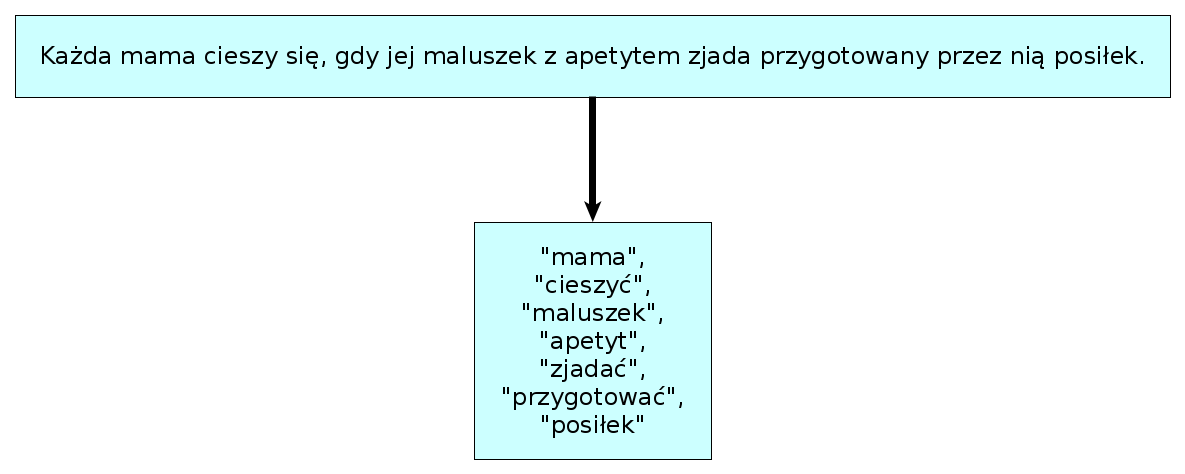
\includegraphics[width=1\textwidth]{img/lemmatisation.png}
		\end{figure}
	\end{frame}
	\section{Metody ewaluacji}
	
	\section{Testy}
	
	\section{Podsumowanie}
	\subsection{Wnioski}
	\subsection{Kiernki dalszych badań}
	\section{Źródła}
	\begin{frame}{Tables and Figures}
		
		\begin{itemize}
			\item Use \texttt{tabular} for basic tables --- see Table~\ref{tab:widgets}, for example.
			\item You can upload a figure (JPEG, PNG or PDF) using the files menu. 
			\item To include it in your document, use the \texttt{includegraphics} command (see the comment below in the source code).
		\end{itemize}
		
		% Commands to include a figure:
		%\begin{figure}
		%\includegraphics[width=\textwidth]{your-figure's-file-name}
		%\caption{\label{fig:your-figure}Caption goes here.}
		%\end{figure}
		
		\begin{table}
			\centering
			\begin{tabular}{l|r}
				Item & Quantity \\\hline
				Widgets & 42 \\
				Gadgets & 13
			\end{tabular}
			\caption{\label{tab:widgets}An example table.}
		\end{table}
		
	\end{frame}

	
\end{document}
